% Exemplo de relatório técnico do IC
% Criado por P.J.de Rezende antes do Alvorecer da História.
% Modificado em 97-06-15 e 01-02-26 por J.Stolfi.
% Last edited on 2003-06-07 21:12:18 by stolfi
% modificado em 1o. de outubro de 2008
% modificado em 2012-09-25 para ajustar o pacote UTF8. Contribuicao de
%   Rogerio Cardoso

\documentclass[11pt,twoside]{article}
\usepackage{techrep-ic}
\usepackage{indentfirst}

%%% SE USAR INGLÊS, TROQUE AS ATIVAÇÕES DOS DOIS COMANDOS A SEGUIR:
\usepackage[brazil]{babel}
%% \usepackage[english]{babel}

%%% SE USAR CODIFICAÇÃO LATIN1, TROQUE AS ATIVAÇÕES DOS DOIS COMANDOS A
%%% SEGUIR:
%% \usepackage[latin1]{inputenc}
\usepackage[utf8]{inputenc}
\usepackage{graphicx}

\begin{document}

%%% PÁGINA DE CAPA %%%%%%%%%%%%%%%%%%%%%%%%%%%%%%%%%%%%%%%%%%%%%%%
%
% Número do relatório
\TRNumber{02}

% DATA DE PUBLICAÇÃO (PARA A CAPA)
%
\TRYear{16}  % Dois dígitos apenas
\TRMonth{04} % Numérico, 01-12

% LISTA DE AUTORES PARA CAPA (sem afiliações).
\TRAuthor{Gabriel Oliveira \and Jo{\~a}o Fid{\'e}lis \and Lucas Morais \and Matheus Figueiredo \and Pedro Grij{\'o}}

% TÍTULO PARA A CAPA (use \\ para forçar quebras de linha).
\TRTitle{MC437 - Grupo06 - Relat{\'o}rio 2}

\TRMakeCover
%%%%%%%%%%%%%%%%%%%%%%%%%%%%%%%%%%%%%%%%%%%%%%%%%%%%%%%%%%%%%%%%%%%%%%
% O que segue é apenas uma sugestão - sinta-se à vontade para
% usar seu formato predileto, desde que as margens tenham pelo
% menos 25mm nos quatro lados, e o tamanho do fonte seja pelo menos
% 11pt. Certifique-se também de que o título e lista de autores
% estão reproduzidos na íntegra na página 1, a primeira depois da
% página de capa.
%%%%%%%%%%%%%%%%%%%%%%%%%%%%%%%%%%%%%%%%%%%%%%%%%%%%%%%%%%%%%%%%%%%%%%

%%%%%%%%%%%%%%%%%%%%%%%%%%%%%%%%%%%%%%%%%%%%%%%%%%%%%%%%%%%%%%%%%%%%%%
% Nomes de autores ABREVIADOS e titulo ABREVIADO,
% para cabeçalhos em cada página.
%
\markboth{Bueno, Fid{\'e}lis, Figueiredo, Grij{\'o}, Morais}{MC437 - Grupo06}
\pagestyle{myheadings}

%%%%%%%%%%%%%%%%%%%%%%%%%%%%%%%%%%%%%%%%%%%%%%%%%%%%%%%%%%%%%%%%%%%%%%
% TÍTULO e NOMES DOS AUTORES, completos, para a página 1.
% Use "\\" para quebrar linhas, "\and" para separar autores.
%
\title{MC437 - Grupo06}

\author{Gabriel Bueno de Oliveira \and
Jo{\~a}o Guilherme Daros Fid{\'e}lis \and
Lucas Henrique Morais \and
Matheus Yokoyama Figueiredo \and Pedro Rodrigues Grij{\'o}}
\date{}

\maketitle

%%%%%%%%%%%%%%%%%%%%%%%%%%%%%%%%%%%%%%%%%%%%%%%%%%%%%%%%%%%%%%%%%%%%%%

\begin{abstract}
\setlength{\parindent}{4ex}
Utilizamos o benchmark TPC-W, que modela uma livraria online, atrav\'es de um ambiente controlado, para simular atividades num servidor WEB. Em conjunto com o simulador RBE, que gera tr\^es diferentes perfis de carga (Shopping, Ordering e Browsing), pudemos checar o desempenho do servidor instalado num cluster no IC, ao vermos o n\'umero de WIPS (WEB Interactions per Second) gerados por diferentes cargas.
O relat\'orio refere-se a segunda parte do projeto da disciplina de MC437 (Projeto de Sistemas de Informa\c{c}\~ao) e tem como objetivo realizar testes com dois bancos de dados diferentes, sendo um primário que é replicado para um secundário em hot-standby, testando quais as melhores cargas que o primário consegue atender e depois medir o tempo de recuperação quando o primário é desligado e o secundário promovido.
\end{abstract}

\section{Introdução}
Este trabalho \'e um relat\'orio da segunda parte do projeto da disciplina MC437 - Projeto de Sistemas de Informação. Essa parte foi constituída pela preparação de uma m\'aquina remota com um servidor  webApache Tomcat, utlização de duas máquinas remotas com instâncias de bancos de dados PostgreSQL, uma com um banco atuando como primário e outra com um banco secundário em hot-standby, utilizado para integrar todas essas funcionalidades e fazer um site de compras com dados gerados aleatoriamente.

    Também foi instalado na máquina do web server o aplicativo TPC-W, um benchmark de transa\c{c}\~oes web. Para fazer uso do TPC-W, foi utlizado o RBE (Remote Browser Emulator), que emula conjuntos de clientes que acessam o lado servidor do TPC-W, sendo que este implementa uma livraria digital.
    
    O RBE \'e um simulador escrito completamente em Java que simula o tr\'afego HTTP gerado por um usu\'ario que estivesse acessando o site atrav\'es de um navegador.

    Também utilizamos o HAProxy, que atua como um proxy para aplicações baseadas em TCP e HTTP. Ele oferece alta disponibilidade e balanceamento de carga para servidores web. Neste trabalho, sua função é de detectar falha do banco primário e redirecionar as requisições feitas para o banco secundário, que deve ser promovido a banco primário.

    O TPC-W gera um n\'umero, o WIPS (Web Interactions per Second). O fluxo de trabalho é gerado pelo RBE e pode ser de tr\^es perfis. O perfil de compras (\textit{shopping}), onde 80\% das a\c{c}\~oes são de leitura e 20\% de escrita no banco de dados. O perfil de navega\c{c}\~ao (\textit{browsing}), tem 95\% das a\c{c}\~oes de leitura e 5\% de escrita. J\'a o perfil de compras (\textit{ordering}) tem 50\% de suas opera\c{c}\~oes de leitura e 50\% de escrita.

    Rodamos três experimentos diferentes, o primeiro apenas com o banco primário ativo, o segundo com o primário ligado e o secundário ligado em hot-standby e o terceiro onde na metade do experimento, o primário era desativado para que o secundário pudesse ser promovido.

\setlength{\parindent}{4ex}


\section{Condições Experimentais}
\setlength{\parindent}{4ex}
     Nesta se\c{c}\~ao ser\~ao descritas as configura\c{c}\~oes de hardware e software utilizadas nos experimentos.

     Nesta fase do trabalho contamos com quatro máquinas, todas com a mesma configuração de hardware, fornecidas pelo Instituto de Computação.

     A primeira, denominada CBN6, é onde estão instalados o HAProxy 1.6, Apache Tomcat versão 7 e TPC-W. A máquina CBN6 atua como servidor web.

     Duas máquinas, a dbmaster2 e dbslave2, é onde ficam os bancos de dados primário e secundário, respectivamente. Nelas está instalado o PostgreSQL vers\~ao 9.5.1.

     Já o RBE foi rodado a partir de outra máquina, a CBN7.

     Todas as máquinas tem a mesma configuração: sistema operacional Ubuntu 14.04, CPU Intel(R) Core(TM)2 Quad CPU Q8400 2.66GHz e mem\'oria RAM de 4GB e 1333 MHz.

\section{Metodologia de Pesquisa}
\setlength{\parindent}{4ex}
Foram executados três diferentes experimentos. Cada experimento consistiu em rodar o RBE para simular uma carga no servidor, e após isso foram avaliadas as medições realizadas pelo RBE.

No primeiro experimento, o RBE foi utilizado com apenas o banco primário ligado. No segundo experimento, estavam ligados o banco primário e o banco secundário em hot-standby.

Esses dois experimentos foram feitos para caracterizar o servidor. O objetivo foi medir a maior carga para a qual ele se comporta de forma consistente.

Para isso, variamos os valores de carga entre 2000 e 4000 clientes, variando de 1000 em 1000 para cada iteração para cada perfil de usuário descrito anteriormente. Assim,  gráficos foram gerados para demonstrar até qual carga o servidor se manteve num bom nível de WIPS ao longo de todo o teste (que dura 100s no total).

O valor encontrado foi utilizado no RBE para simular essa "carga ótima" no servidor, causando um failover manualmente (isto é, matando o banco de dados primário), enquanto o banco de dados secundário era promovido, para ver em quanto tempo o servidor conseguia se recuperar e voltar a ficar ativo.

É importante ressaltar que o RBE sempre foi RBE de outra máquina remota (CBN7), diferente de da máquina do servidor(CBN6), e que os parâmetros utilizados foram Ramp-Up Time: 5s, Ramp-Down Time: 5s e Measurement Interval: 90s. O valor de máximo número de erros tolerados foi colocado em 0. Todos os outros valores são os padrões do RBE.

\section{An\'alise e Resultados}
\setlength{\parindent}{4ex}

Seguem os gráficos gerados pela execução do RBE para o experimento 1.
\begin{center}
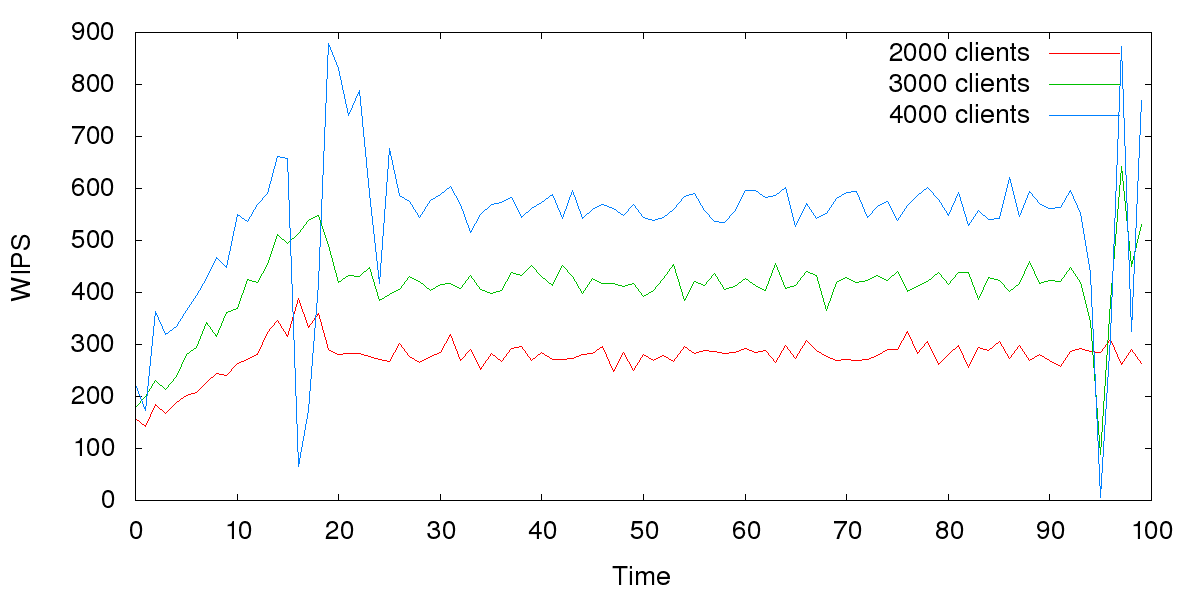
\includegraphics[width=15cm, height=10cm]{images/exp1/plot_browsin}
Figura 1: WIPS por tempo(s) para cada carga simulada pelo RBE no perfil Browsing do experimento 1
\end{center}
Nota-se que o experimento com 4000 clientes teve uma boa consistência entre 30 e 90 segundos, porém houve uma grande queda por volta dos 15s e a partir dos 90s. O mesmo ocorreu no caso para 3000 clientes a partir de 90s.

\begin{center}
\vspace{-1em}
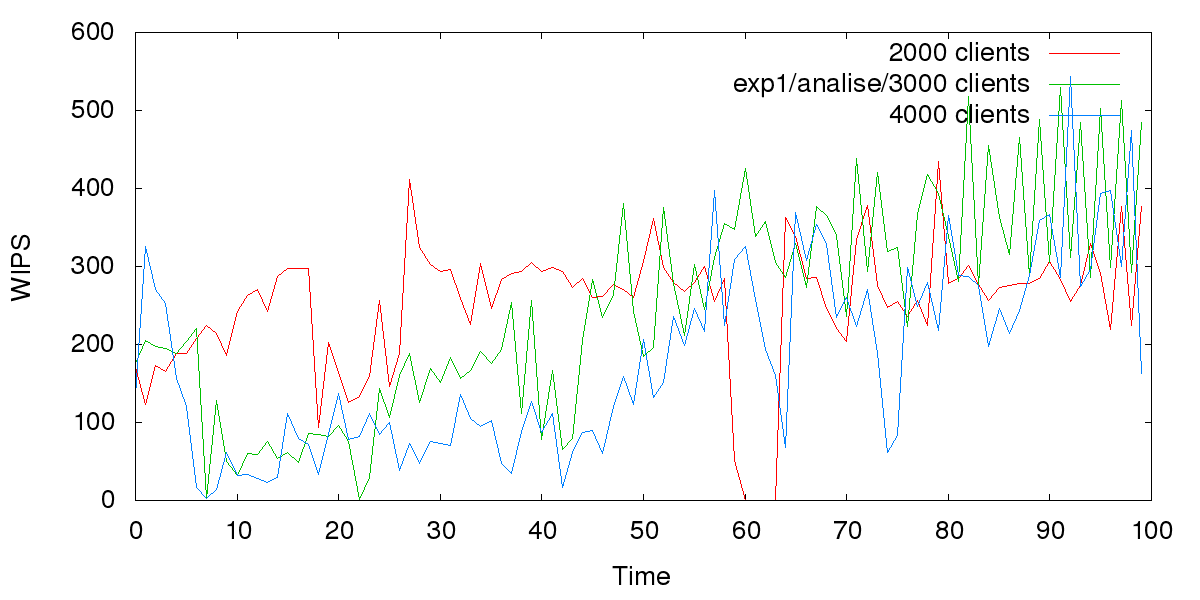
\includegraphics[width=15cm, height=10cm]{images/exp1/plot_ordering}
Figura 2: WIPS por tempo(s) para cada carga simulada pelo RBE no perfil Ordering do experimento 1
\end{center}
Pelo gráfico, é visível que o teste com 3000 clientes obteve o melhor desempenho no geral. Até 50s, o desempenho era melhor com 2000 clientes, porém após esse tempo o teste com 3000 clientes obteve uma quantidade maior de WIPS e se manteve consistentemente melhor que os testes com 2000 e 4000 clientes. 

\begin{center}
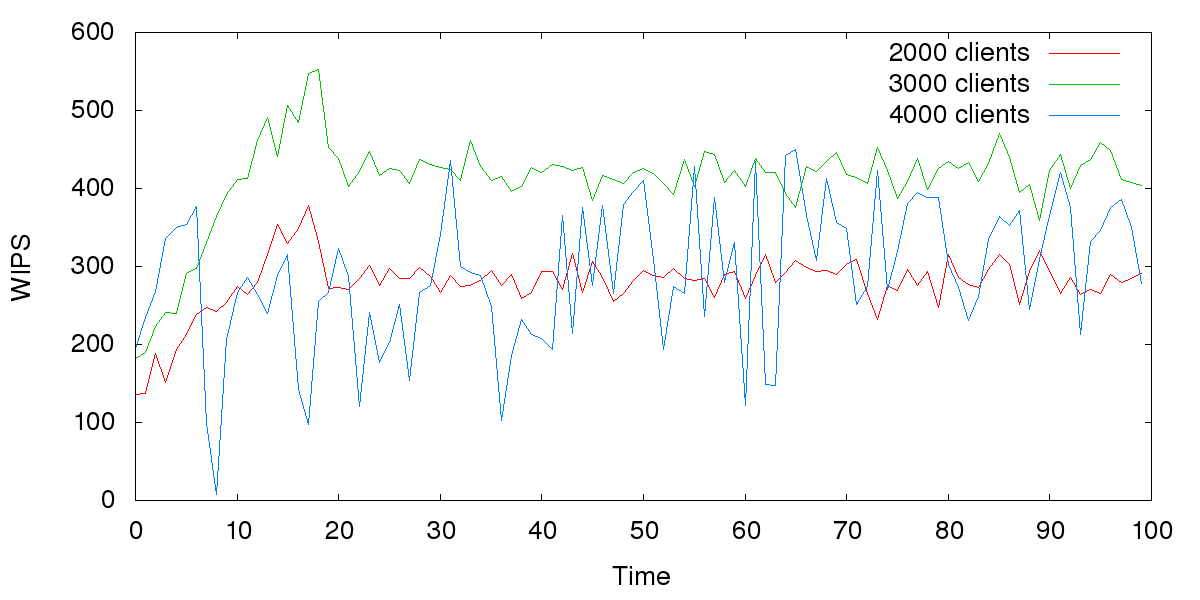
\includegraphics[width=15cm, height=10cm]{images/exp1/plot_shopping}
Figura 3: WIPS por tempo(s) para cada carga simulada pelo RBE no perfil Shopping do experimento 1
\end{center}

Neste gráfico, ficou evidente o melhor desempenho da simulação com 3000 clientes sobre as duas outras. Uma melhor taxa de WIPS foi obtida durante praticamente todo o experimento.

Com a combinação dos resultados desses gráficos, temos indícios de que 3000 usuários talvez seja o melhor número a ser utilizado, pois tem taxas de WIPS mais altas e estáveis que as outras quantidades de usuários testadas.

Agora, analisaremos os dados do experimento 2.

\begin{center}
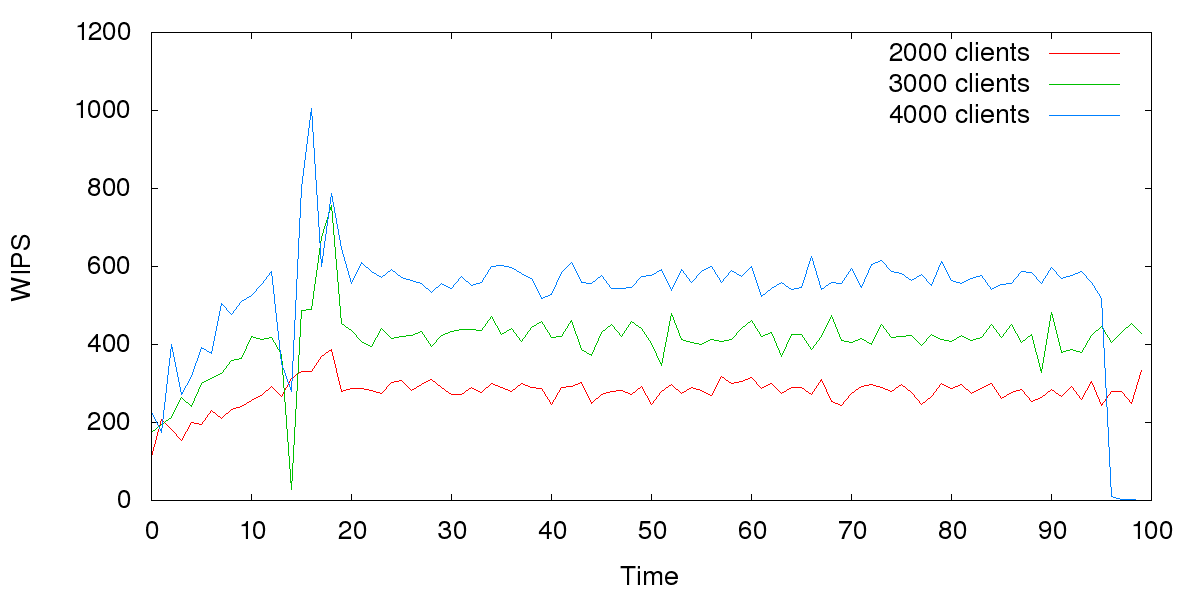
\includegraphics[width=15cm, height=10cm]{images/exp2/plot_browsin}
Figura 4: WIPS por tempo(s) para cada carga simulada pelo RBE no perfil Browsing do experimento 2
\end{center}

O gráfico indica um melhor desempenho geral para 4000 clientes. Entretanto, no final do experimento há uma grande queda, que indica problemas devido a alta carga. Nesse caso, 3000 clientes apresenta melhor estabilidade em relação a 4000 e maior quantidade de WIPS em relação a 2000 clientes

\begin{center}
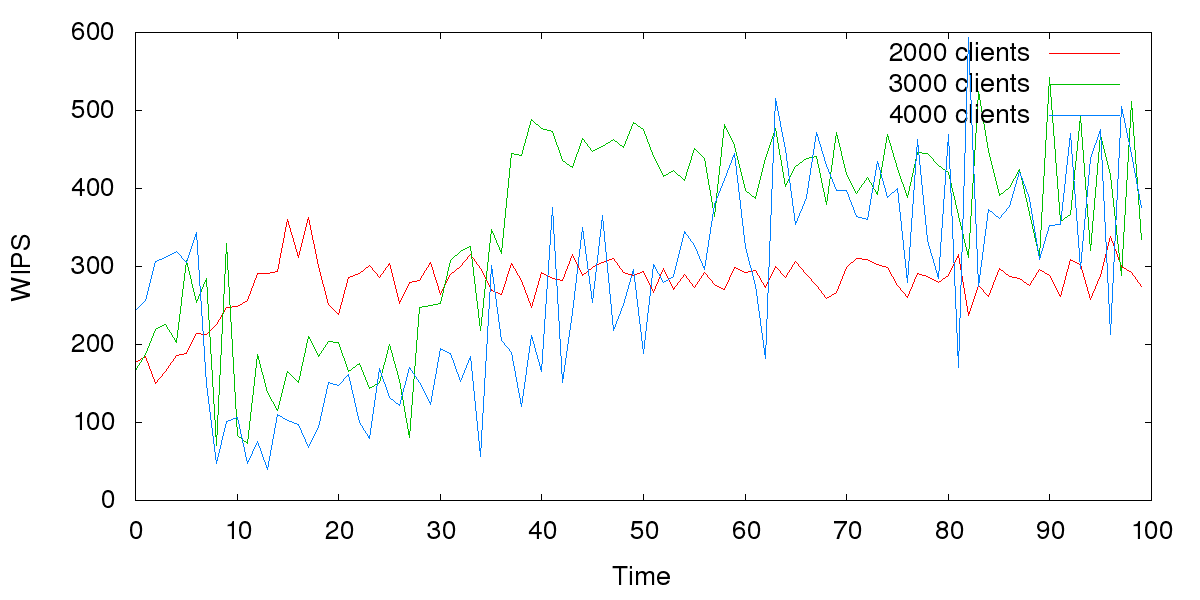
\includegraphics[width=15cm, height=10cm]{images/exp2/plot_ordering}
Figura 5: WIPS por tempo(s) para cada carga simulada pelo RBE no perfil Ordering do experimento 2
\end{center}

O melhor desempenho geral foi para 3000 clientes, pois essa carga manteve uma boa média durante todo o experimento e se manteve no mesmo nível de WIPS para 4000 clientes na segunda metade do experimento.

\begin{center}
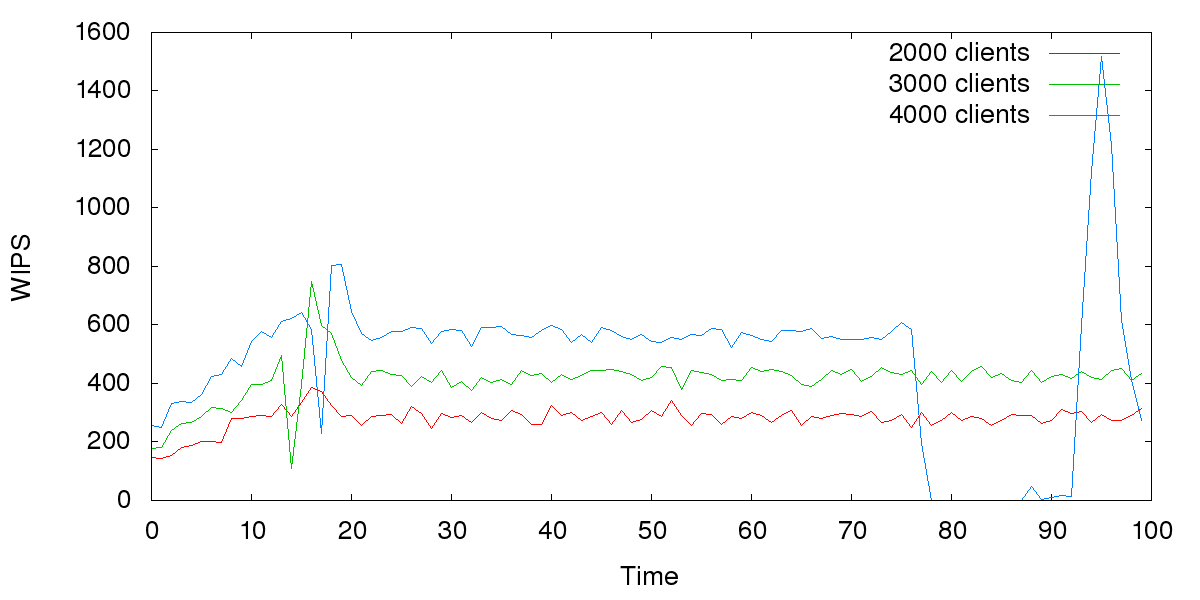
\includegraphics[width=15cm, height=10cm]{images/exp2/plot_shopping}
Figura 6: WIPS por tempo(s) para cada carga simulada pelo RBE no perfil Shopping do experimento 2
\end{center}

Este resultado se assemelha ao do perfil Browsing. 4000 clientes possui bom desempenho até ~70s do experimento, quando sofre queda de WIPS, o que indica que esta alta carga sobrecarrega o servidor. Como no perfil Browsing, a carga mais estável é de 3000 clientes.

\section{Conclus\~ao}

\end{document}
